\chapter{Budućnost Fundamentalnih Principa}

Već smo pročitali sljedeći citat iz poglavlja “\textit{Temelj Naše Vjere}”. To je jedno od proročkih viđenja sestre White o velikoj reformi koja će se dogoditi među Adventistima Sedmog Dana; ta reforma će se sastojati u odricanju od Fundamentalnih Principa. To je upravo način na koji će se uspostaviti nova organizacija.

\egw{\textbf{Neprijatelj duša tražio je da uvede pretpostavku da će nastati velika reformacija među Adventistima Sedmog Dana, i da će se ta reforma \underline{sačinjavati od odstupanja od doktrina koje stoje kao stupovi naše vjere} i da će se pokrenuti proces reorganizacije}. Kada bi takva reformacija nastupila, kakav bi bio rezultat? \textbf{Principi istine koje Bog u svojoj mudrosti dao crkvi ostatka bili bi odbačeni. Naša religija bi se promijenila. \underline{Fundamentalni principi koji su održavali posao posljednjih pedeset godina bili bi proglašeni greškom}}. \textbf{Nova organizacija bi se osnovala. Knjige novog reda bi se napisale. Uveo bi se sistem intelektualne filozofije}. Osnivači ovog pokreta išli bi u gradove i napravili nevjerojatan posao. Naravno, subota bi se olako smatrala, kao i Bog koji ju je stvorio. Ničemu ne bi bilo dopušteno stajati na putu novom pokretu. Vođe bi poučavali da je vrlina bolja od poroka, ali \textbf{kako je Bog uklonjen}, oni će \textbf{staviti svoju ovisnost na ljudske snage} koje su, bez Boga, bezvrijedne. Njihov temelj će biti izgrađen na pijesku, a oluja i bura će odnijeti strukturu.}[Lt242-1903.13; 1903][https://egwwritings.org/read?panels=p7767.20]

\egwnogap{Tko ima ovlasti započeti takav pokret? \textbf{Imamo naše Biblije. Imamo svoje iskustvo koje je potvrđeno čudesnim radom Duha Svetoga}. \textbf{Imamo istinu koja ne prihvaća kompromise.} \textbf{\underline{Ne bismo li trebali odbaciti sve što nije u skladu s tom istinom}?}}[Lt242-1903.14; 1903][https://egwwritings.org/read?panels=p7767.21]

Ellen White je vidjela napore neprijatelja da ukloni ove \emcap{Fundamentalne Principe}. Oni su održali rad od samog početka. Bile su to istine potvrđene čudesnim djelovanjem Duha Svetoga i ne dopuštaju nikakav kompromis. \egwinline{Ne bismo li trebali odbaciti sve što nije u skladu s tom istinom?}

\begin{figure}
    \centering
    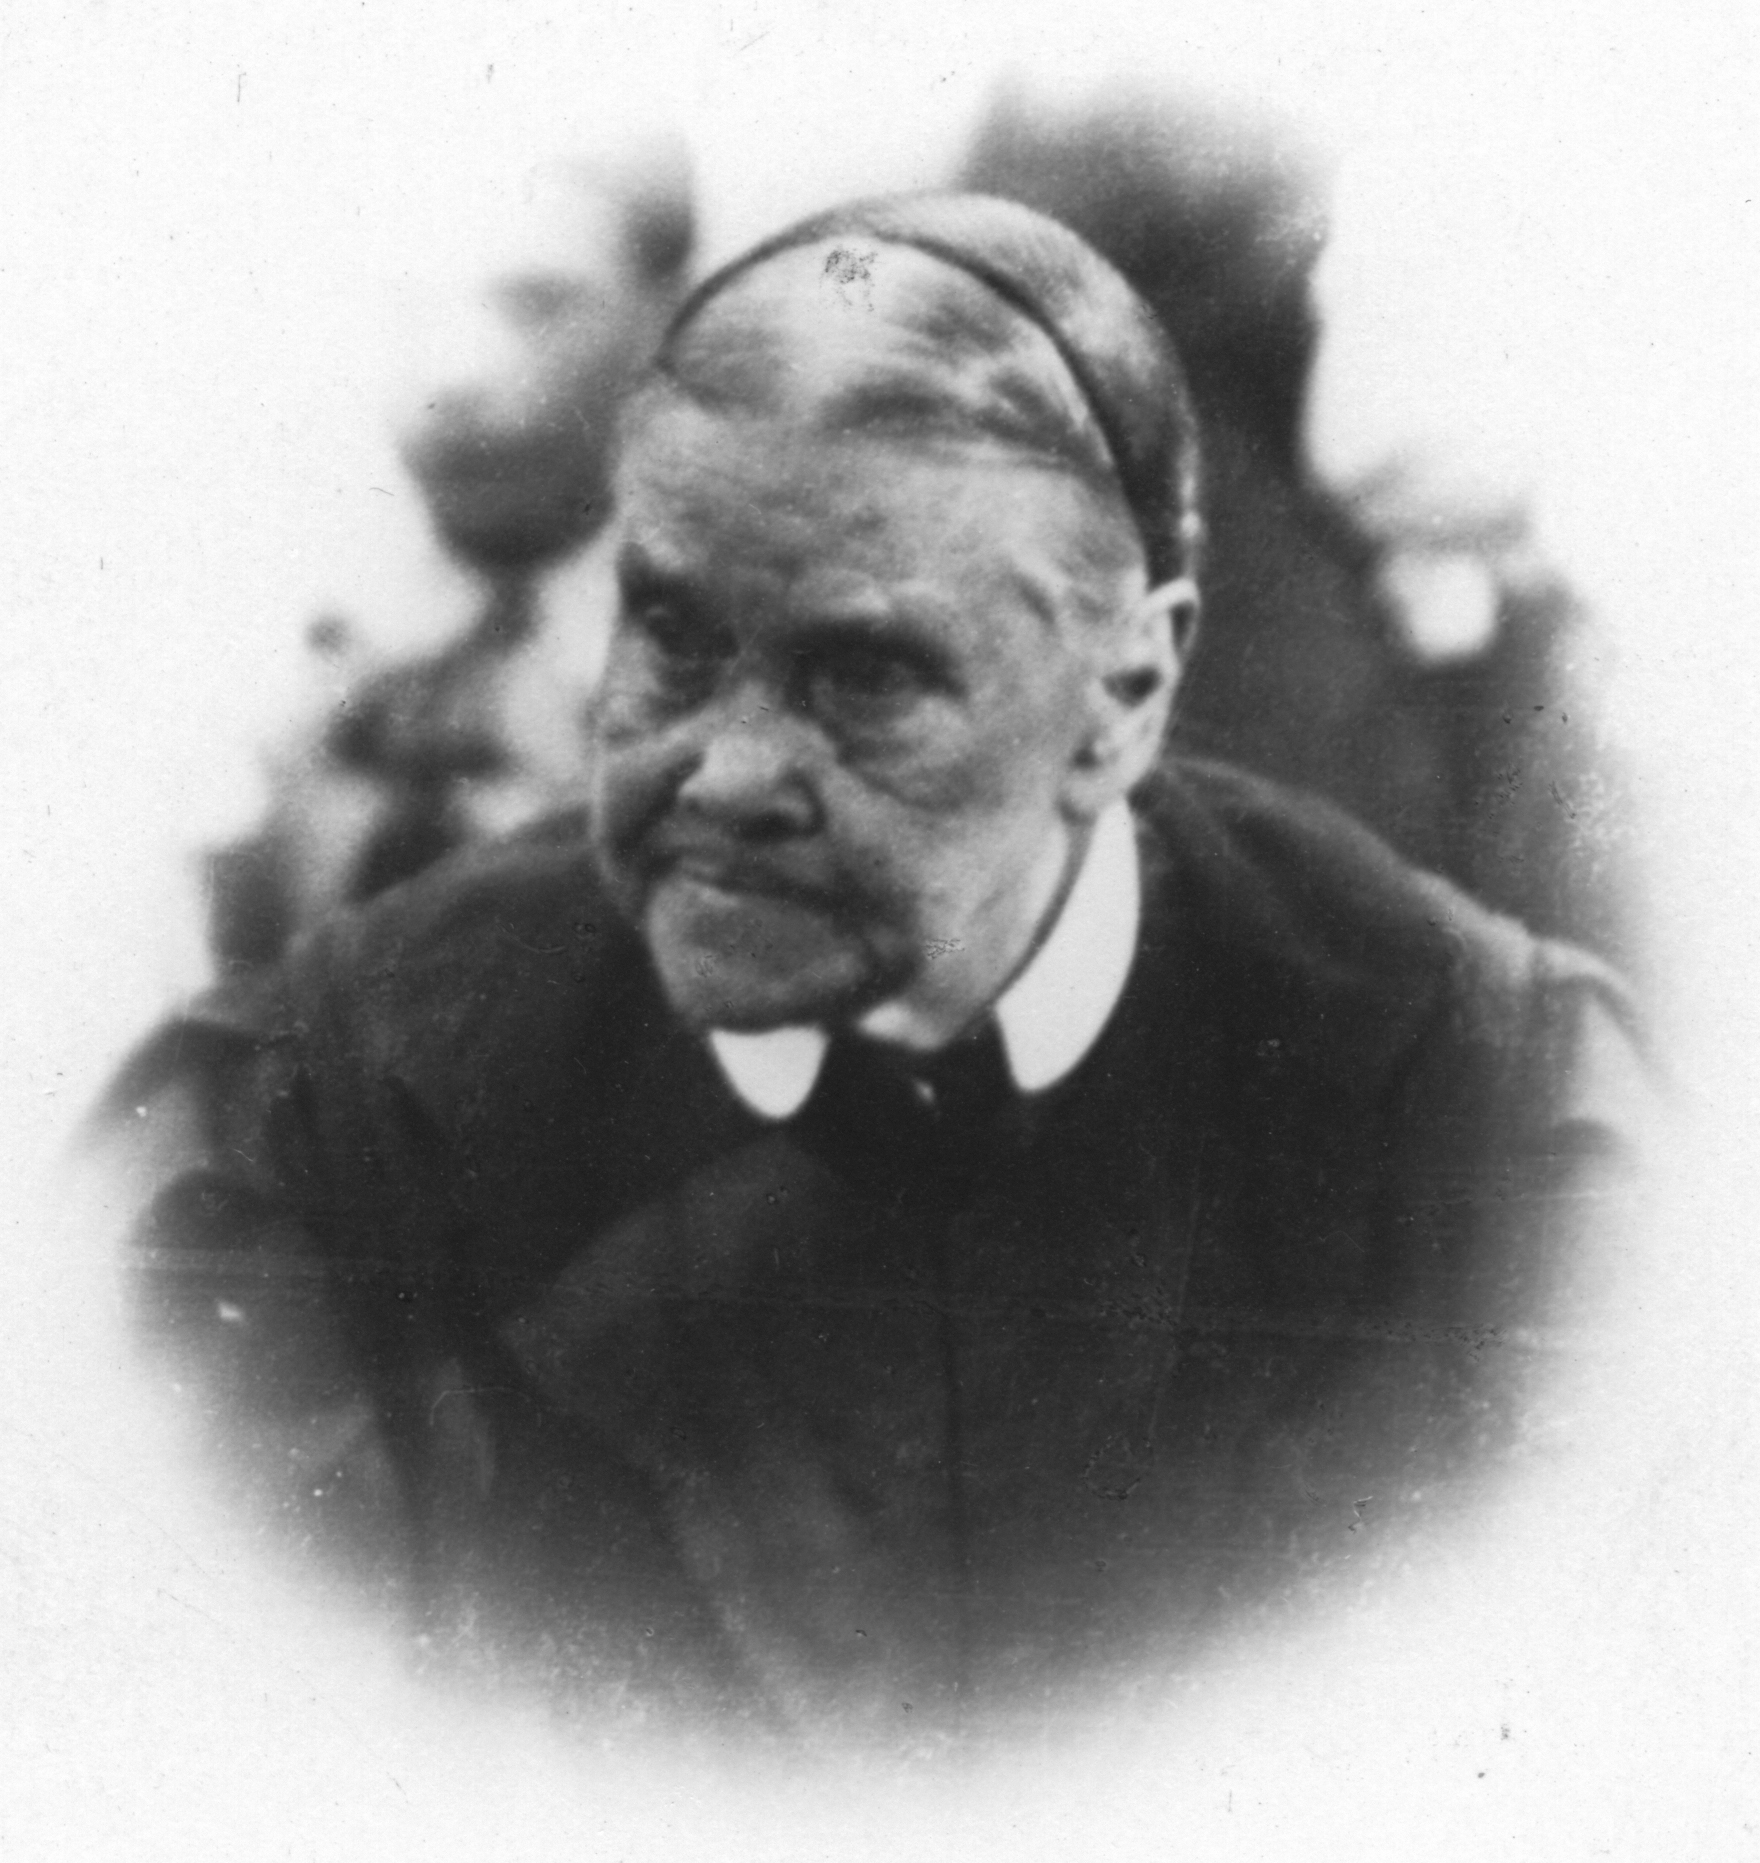
\includegraphics[width=1\linewidth]{images/ellen-white-1913.jpg}
    \caption*{Ellen G. White, 1913}
    \label{fig:e-white-1913}
\end{figure}

Sestra White nam je prorekla budućnost. Danas svjedočimo njenom ispunjenju. Uspoređujući \emcap{Fundamentalne Principe} s današnjim Temeljnim Vjerovanjima, vidimo da se naša religija promijenila. Naše vjerovanje o \emcap{ličnosti Boga} se promijenilo. Knjige novog reda su napisane, koje nisu utemeljene na čvrstoj Riječi Božjoj. Uveden je sustav intelektualne filozofije.

Ova reforma se dogodila u njezino vrijeme. Ovako je opisala dane Crkve Adventista Sedmog Dana u svoje vrijeme i u budućnosti:

\egw{Sadašnje vrijeme je svečano, zastrašujuće vrijeme za crkvu. Anđeli su već opasani, čekajući zapovijed Božju da izliju svoje čaše gnjeva na svijet. Anđeli zatirači započinju djelo osvete, jer se Duh Božji postupno povlači iz svijeta. Sotona također okuplja svoje snage zla, izlazeći ‘kraljevima zemlje i cijelog svijeta’, da ih skupi pod svoj barjak, da ih obuči za ‘bitku onoga velikog dana Svemogućeg Boga.’ \textbf{Sotona će uložiti najmoćnije napore za prevlast u posljednjem velikom sukobu. \underline{Fundamentalni Principi će biti izneseni, i odluke donesene u vezi s njima}. Skepticizam prevladava posvuda}. Bezakonje obiluje. \textbf{Vjera pojedinačnih članova crkve bit će testirana kao da nema druge osobe na svijetu}...}[Ms1a-1890.8; 1890][https://egwwritings.org/read?panels=p6780.13]

Sotonini najmoćniji napori usmjereni su na uklanjanje \emcap{Fundamentalnih Principa} obavijajući ih skepticizmom. Sudeći prema današnjoj perspektivi, svjedočimo istinitosti proročanstava Ellen White.

\egw{Kažem vam sada, da kada budem položena na počinak, \textbf{dogodit će se velike promjene}.}[Ms1-1915.2; 1915][https://egwwritings.org/read?panels=p10771.9]

Pravo pitanje koje imamo za sebe je, kada se \emcap{Fundamentalni Principi} iznesu, koju odluku ću donijeti u vezi s njima? Zar ne bismo trebali odbaciti sve što nije u skladu s tim principima? Koju odluku ćeš donijeti?

% Budućnost Fundamentalnih Principa

\begin{titledpoem}

    \stanza{
        Nakon smrti moje, promjene će doći, \\
        Ellen White je rekla u proročkoj moći. \\
        Danas vidimo da riječi njene žive, \\
        Dok se stare istine pod novim velom skrile.
    }

    \stanza{
        Skepticizam raste, vjera se mijenja, \\
        Sotonina vojska već se sprema. \\
        Principi istine na kušnji stoje, \\
        Dok anđeli Božji čaše gnjeva broje.
    }

    \stanza{
        Sustav filozofije intelektualne, \\
        Zamjenjuje istine fundamentalne. \\
        Imamo Biblije, imamo iskustvo, \\
        Potvrde Duha Svetog naše je jamstvo.
    }

    \stanza{
        Što ćeš učiniti kad se principi iznesu? \\
        Hoćeš li stajati čvrsto u tom stresu? \\
        Vjera će se kušati kao nikad prije, \\
        Kao da na svijetu nitko drugi nije.
    }

    \stanza{
        Odluka je tvoja, vrijeme je sada, \\
        Kad se temelj vjere pred tobom raspada. \\
        Vrati se izvorima, čvrsto stoj, \\
        Za Fundamentalne Principe bij boj.
    }
    
\end{titledpoem}